\section{The Alchemist Metamodel}\label{sec:the-alchemist-metamodel}

As for the implementation of the simulation, the \textit{Alchemist Simulator}~\cite{Pianini_2013} was used for the following reasons:
\begin{itemize}
    \item It provides a \textit{ready-to-use} simulation environment, avoiding to implement one from scratch.
    \item It provides an intuitive graphic user interface that allows observing the evolution of the developed simulation.
    \item To contribute to the \textit{research and development} area of the \textit{Dipartimento di Informatica - Scienze e Ingegneria} (\textit{DISI}) of the \textit{University of Bologna}.
\end{itemize}

\noindent
\textit{Alchemist} presents its own metamodel, providing a series of concepts necessary to be understood in order to develop a simulation.
In this section, only the crucial aspects will be reported, in order to fully understand the current simulation; for further information, please check the~\href{https://alchemistsimulator.github.io/}{official documentation}.
The main entities of the metamodel are:
\begin{itemize}
    \item \textbf{Molecule}: the name of a data item; it can be seen as a variable name.
    \item \textbf{Concentration}: the value associated to a specific molecule.
    \item \textbf{Node}: a container of molecules and reactions.
    \item \textbf{Environment}: the space abstraction that contains nodes and provides them with spatial capabilities (position, movement, etc.).
    \item \textbf{Linking Rule}: a function of the environment that associates a node with others.
    \item \textbf{Reaction}: an event that can change the status of the environment.
\end{itemize}

\noindent
The image \ref{fig:model} provides a visual representation of such metamodel:
\begin{figure}[H]
    \centering
    \includegraphics[width=.8\textwidth]{../img/model}
    \caption{Visual representation of the \textit{Alchemist} metamodel.}
    \label{fig:model}
\end{figure}

\noindent
The \textit{Alchemist} metamodel is implemented by different \textbf{incarnations}, that is to say, concrete instances of the metamodel.
Among the different incarnations, the~\href{https://protelis.github.io/}{Protelis Incarnation} was chosen, as it seems to be the one that better adapts to the current simulation.
\textit{Protelis} is a domain-specific language for \textit{aggregate programming}. \textit{Aggregate programming} produces reliable and robust collective behavior from uncoordinated local interactions between nodes, and provides higher-level abstractions for device-to-device communication and aggregate-level operations for distributed coordination~\cite{protelis}.
